\section{Derivatives}
Let $f$ be a function of one variable. What is the difference between the derivative of that function and the partial derivative? See SICM p.26-27.

\section{Separation of variables}
In order to solve certain differential equations we sometimes write acceleration as
\begin{align*}
  \frac{\d v}{\dt} = \frac{\d v}{\dx}\frac{\dx}{\dt} = v \frac{\d v}{\dx}.
\end{align*}
How does one think about that? Is there an intuitive way of thinking about the mathematical fact
that the rate of change of velocity over time is equal to velocity multiplied by the rate of change
of velocity over space?

\begin{mdframed}
  Suppose at $t=0$ a particle is at position $x=0$ and has velocity $v=0$. It now accelerates at a
  constant rate $c$. So we have
  \begin{align*}
    \dvdt &= c \\
    \dxdt &= ct \\
    x(t) &= \frac{1}{2}ct^2
  \end{align*}

\end{mdframed}

\section{Work, friction}
Show that work depends on path in presence of friction.

\section{Harmonic oscillation}

Simple harmonic oscillation without damping is described by the differential equation
\begin{align*}
  \ddot{x} = -kx,
\end{align*}
and the solution is presented in the book as the set of linear combinations of complex exponential
basis functions:
\begin{align*}
  x(t) = Ae^{i\omega t} + Be^{-i\omega t},
\end{align*}
where $\omega \in \R$.

But in general, such an $x(t)$ is complex-valued, whereas the physical problem requires a
real-valued solution.

In the case of ``underdamped'' harmonic motion, the book is explicit that restrictions must be
placed on $A$ and $B$ to ensure real solutions (and implies that $A$ and $B$ are complex):

\begin{mdframed}
  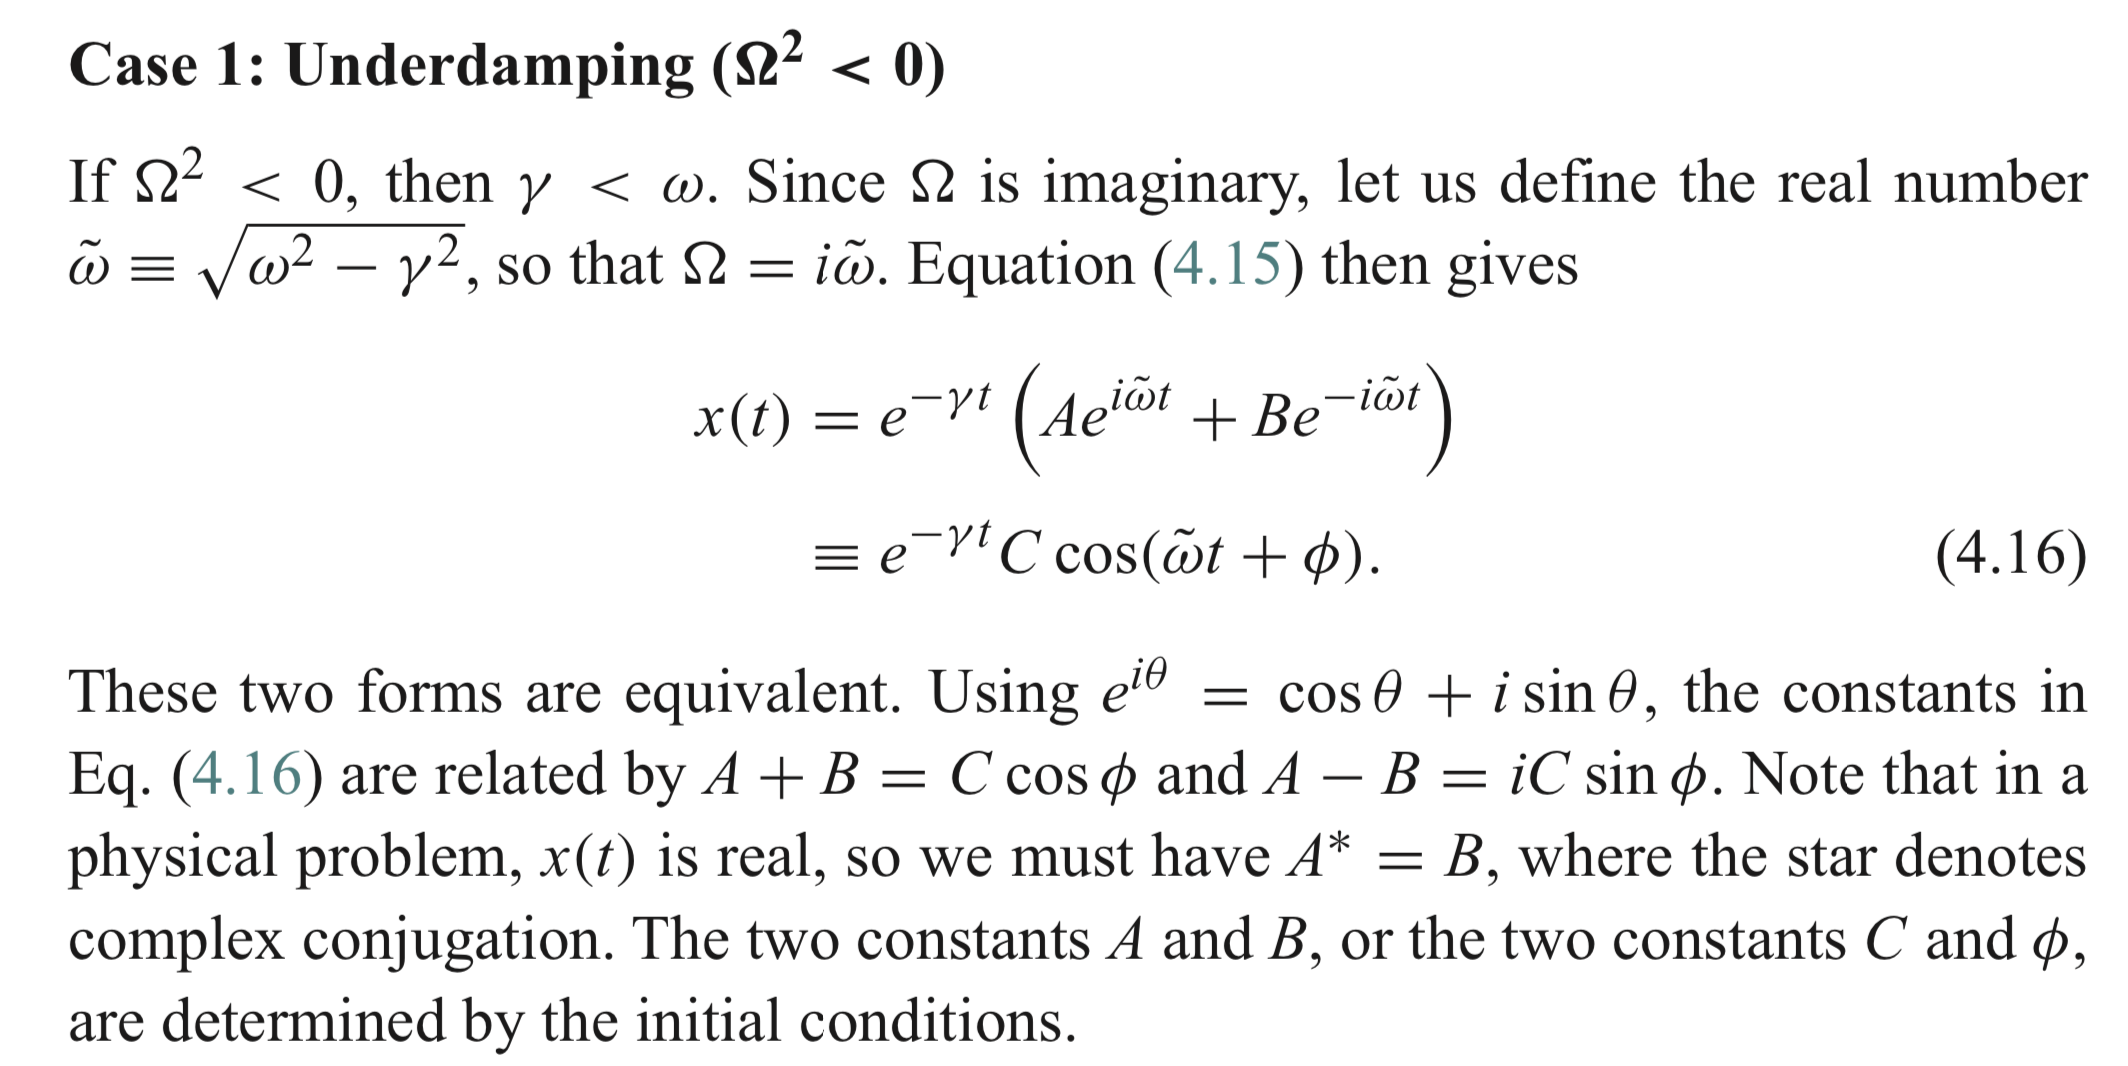
\includegraphics[width=300pt]{img/physics--classical-mechanics--morin--questions--4-3-underdamped-shm.png}
\end{mdframed}

However, in the case of undamped harmonic motion, the book seems not to do this, and as far as I can
see gives inconsistent real and complex versions of the solution:

\begin{mdframed}
  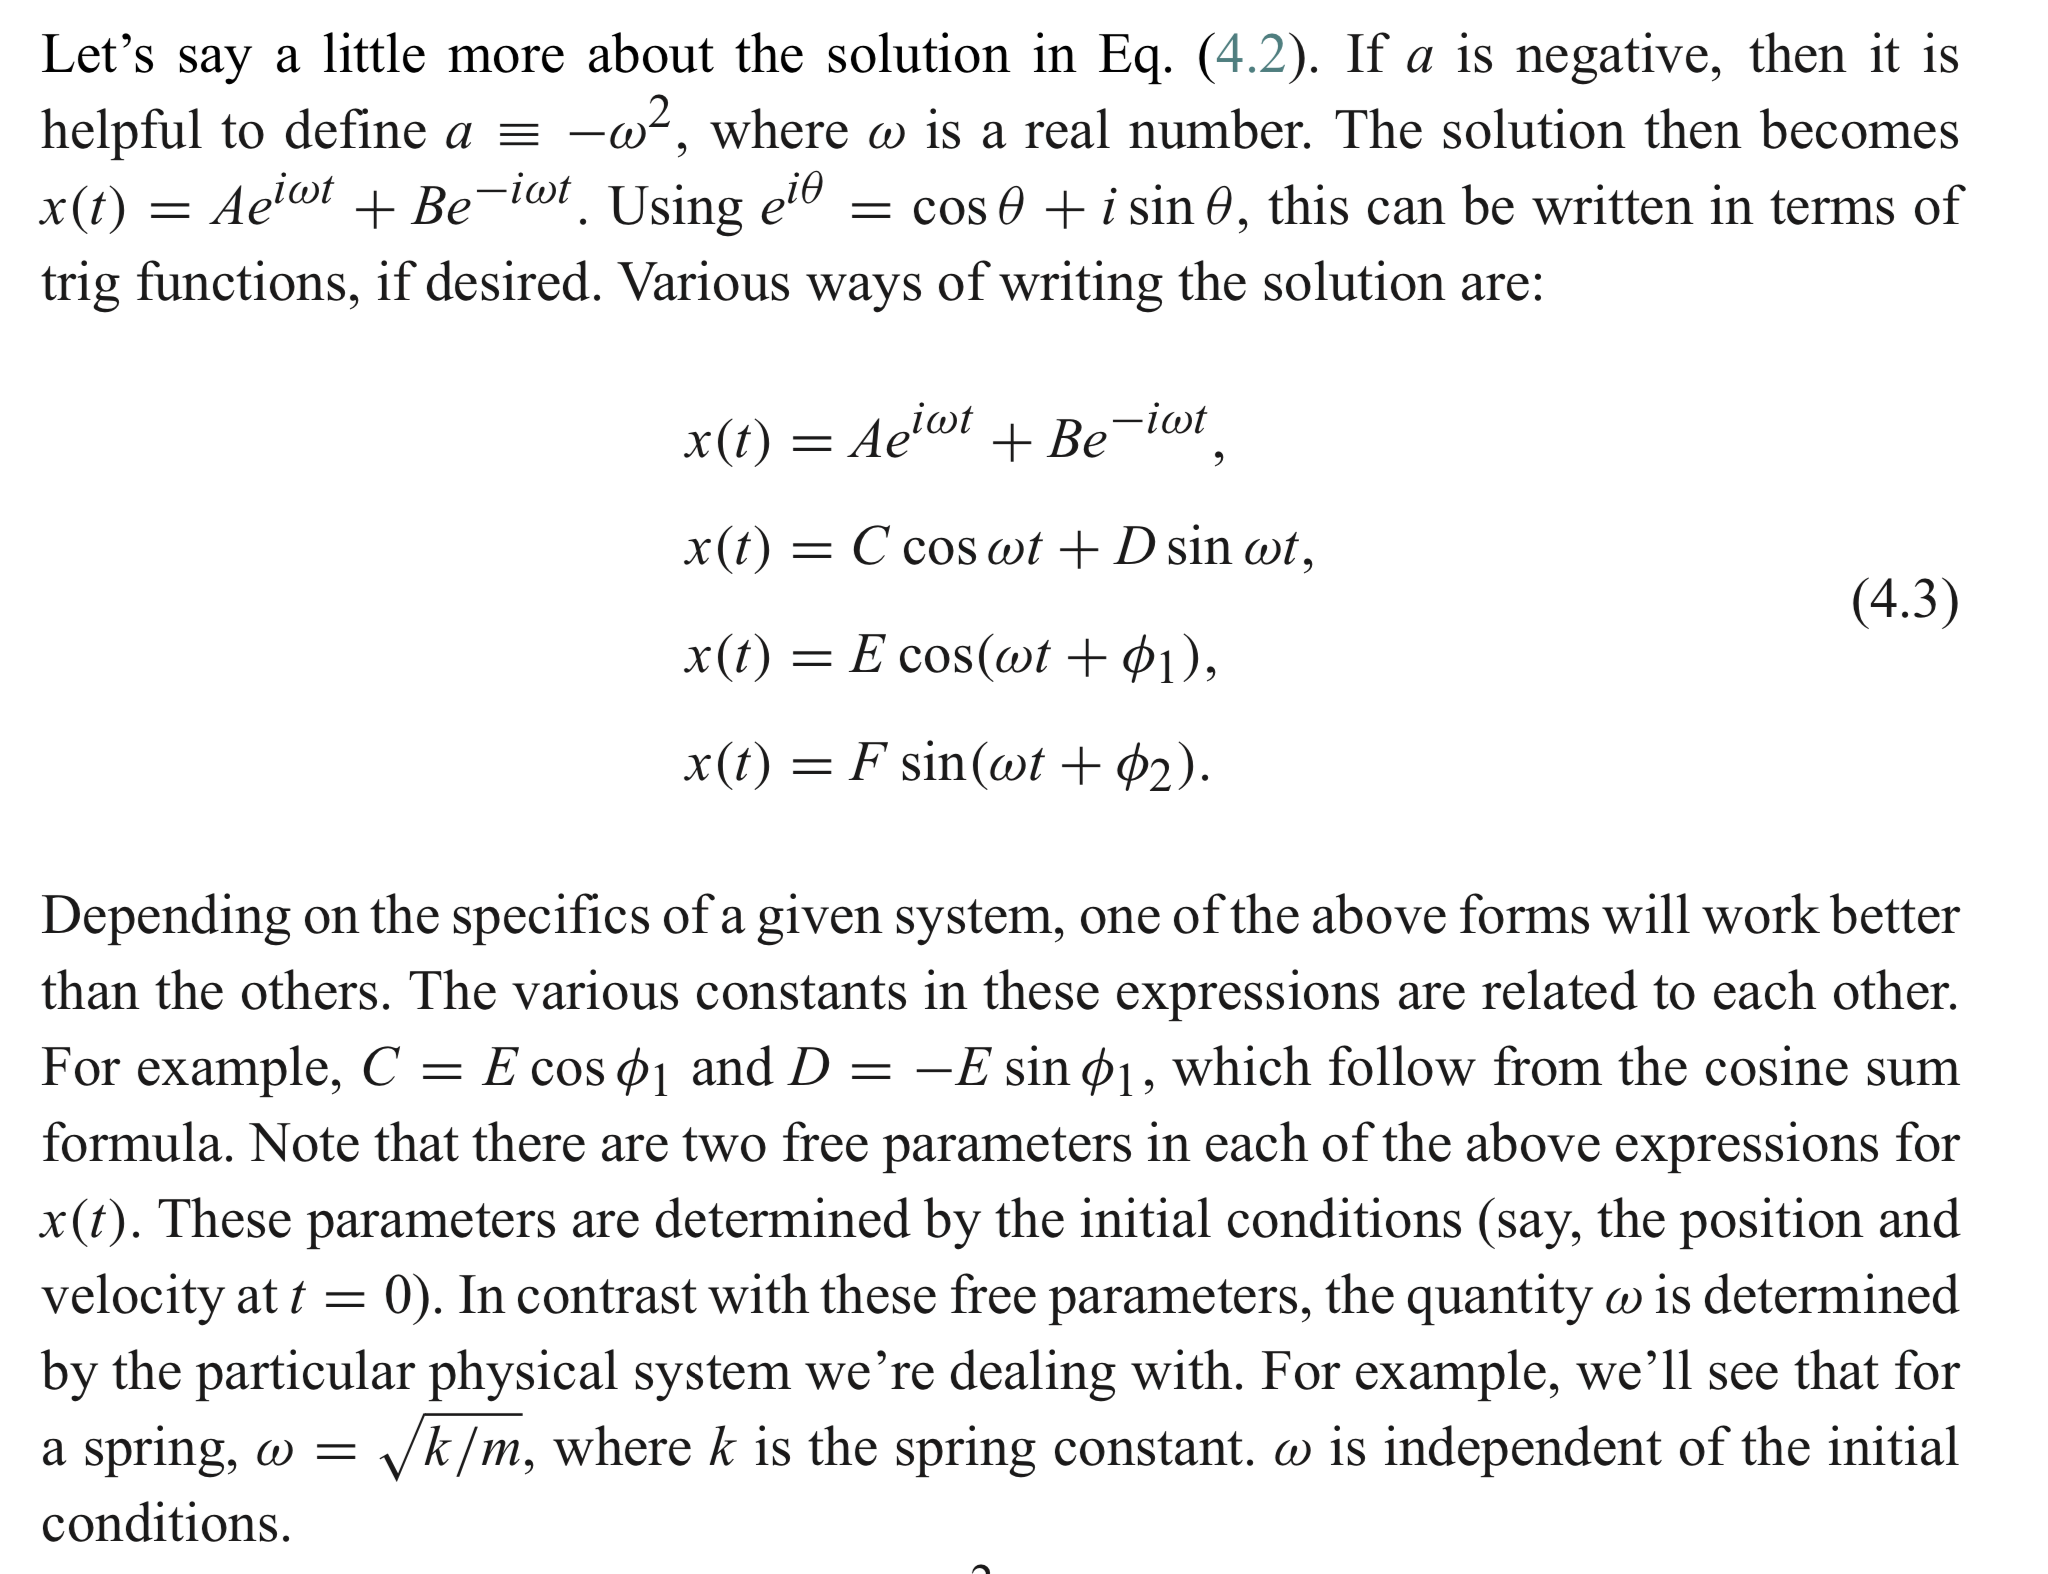
\includegraphics[width=300pt]{img/physics--classical-mechanics--morin--questions--4-3-undamped-shm.png}
\end{mdframed}


\section{Misc}
How much energy does one sit-up require?

body = 164 lbs
upper torso = 80 lbs = 36.3 kg
bag = 36 lbs = 16.3 kg
centre of gravity of body + bag elevated by 0.15 m

work = force x distance
= mgd (kg . m/s/s . m) i.e. Nm
= Cmgd calories where C = 0.239 calories/Nm
